\begin{figure}[H]
  \centering
  \begin{subfigure}[t]{.48\linewidth}
    \centering
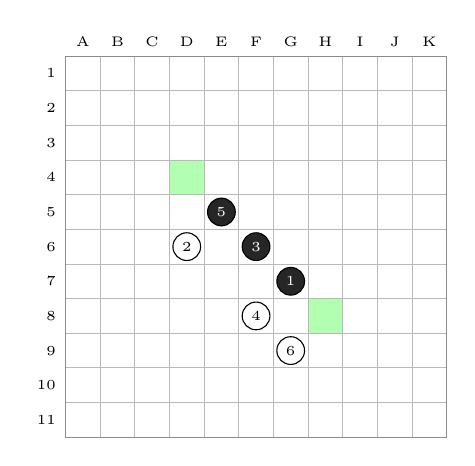
\begin{tikzpicture}[x=0.44cm, y=0.44cm]
\fill[green!30] (3,-3) rectangle (4,-4);
\fill[green!30] (7,-7) rectangle (8,-8);
\draw[gray!55, line width=.3pt, step=1] (0,0) grid (11,-11);
\draw[gray!90] (0,0) rectangle (11,-11);
\node[font=\tiny, anchor=south] at (0.5,0) {A};
\node[font=\tiny, anchor=south] at (1.5,0) {B};
\node[font=\tiny, anchor=south] at (2.5,0) {C};
\node[font=\tiny, anchor=south] at (3.5,0) {D};
\node[font=\tiny, anchor=south] at (4.5,0) {E};
\node[font=\tiny, anchor=south] at (5.5,0) {F};
\node[font=\tiny, anchor=south] at (6.5,0) {G};
\node[font=\tiny, anchor=south] at (7.5,0) {H};
\node[font=\tiny, anchor=south] at (8.5,0) {I};
\node[font=\tiny, anchor=south] at (9.5,0) {J};
\node[font=\tiny, anchor=south] at (10.5,0) {K};
\node[font=\tiny, anchor=east] at (0,-0.5) {1};
\node[font=\tiny, anchor=east] at (0,-1.5) {2};
\node[font=\tiny, anchor=east] at (0,-2.5) {3};
\node[font=\tiny, anchor=east] at (0,-3.5) {4};
\node[font=\tiny, anchor=east] at (0,-4.5) {5};
\node[font=\tiny, anchor=east] at (0,-5.5) {6};
\node[font=\tiny, anchor=east] at (0,-6.5) {7};
\node[font=\tiny, anchor=east] at (0,-7.5) {8};
\node[font=\tiny, anchor=east] at (0,-8.5) {9};
\node[font=\tiny, anchor=east] at (0,-9.5) {10};
\node[font=\tiny, anchor=east] at (0,-10.5) {11};
\draw[fill=black!85, line width=.4pt] (4.5,-4.5) circle (.40);
\node[font=\tiny, text=white, inner sep=0pt] at (4.5,-4.5) {5};
\draw[fill=white, line width=.4pt] (3.5,-5.5) circle (.40);
\node[font=\tiny, text=black, inner sep=0pt] at (3.5,-5.5) {2};
\draw[fill=black!85, line width=.4pt] (5.5,-5.5) circle (.40);
\node[font=\tiny, text=white, inner sep=0pt] at (5.5,-5.5) {3};
\draw[fill=black!85, line width=.4pt] (6.5,-6.5) circle (.40);
\node[font=\tiny, text=white, inner sep=0pt] at (6.5,-6.5) {1};
\draw[fill=white, line width=.4pt] (5.5,-7.5) circle (.40);
\node[font=\tiny, text=black, inner sep=0pt] at (5.5,-7.5) {4};
\draw[fill=white, line width=.4pt] (6.5,-8.5) circle (.40);
\node[font=\tiny, text=black, inner sep=0pt] at (6.5,-8.5) {6};
\end{tikzpicture}
    \caption{C3-016: X đi; 5/8 tác tử đúng}
  \end{subfigure}\hfill
  \begin{subfigure}[t]{.48\linewidth}
    \centering
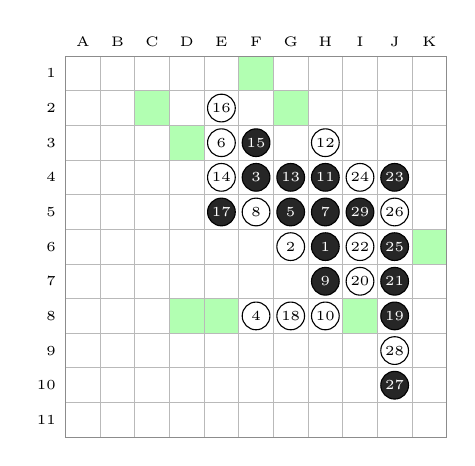
\begin{tikzpicture}[x=0.44cm, y=0.44cm]
\fill[green!30] (5,0) rectangle (6,-1);
\fill[green!30] (2,-1) rectangle (3,-2);
\fill[green!30] (6,-1) rectangle (7,-2);
\fill[green!30] (3,-2) rectangle (4,-3);
\fill[green!30] (10,-5) rectangle (11,-6);
\fill[green!30] (3,-7) rectangle (4,-8);
\fill[green!30] (4,-7) rectangle (5,-8);
\fill[green!30] (8,-7) rectangle (9,-8);
\draw[gray!55, line width=.3pt, step=1] (0,0) grid (11,-11);
\draw[gray!90] (0,0) rectangle (11,-11);
\node[font=\tiny, anchor=south] at (0.5,0) {A};
\node[font=\tiny, anchor=south] at (1.5,0) {B};
\node[font=\tiny, anchor=south] at (2.5,0) {C};
\node[font=\tiny, anchor=south] at (3.5,0) {D};
\node[font=\tiny, anchor=south] at (4.5,0) {E};
\node[font=\tiny, anchor=south] at (5.5,0) {F};
\node[font=\tiny, anchor=south] at (6.5,0) {G};
\node[font=\tiny, anchor=south] at (7.5,0) {H};
\node[font=\tiny, anchor=south] at (8.5,0) {I};
\node[font=\tiny, anchor=south] at (9.5,0) {J};
\node[font=\tiny, anchor=south] at (10.5,0) {K};
\node[font=\tiny, anchor=east] at (0,-0.5) {1};
\node[font=\tiny, anchor=east] at (0,-1.5) {2};
\node[font=\tiny, anchor=east] at (0,-2.5) {3};
\node[font=\tiny, anchor=east] at (0,-3.5) {4};
\node[font=\tiny, anchor=east] at (0,-4.5) {5};
\node[font=\tiny, anchor=east] at (0,-5.5) {6};
\node[font=\tiny, anchor=east] at (0,-6.5) {7};
\node[font=\tiny, anchor=east] at (0,-7.5) {8};
\node[font=\tiny, anchor=east] at (0,-8.5) {9};
\node[font=\tiny, anchor=east] at (0,-9.5) {10};
\node[font=\tiny, anchor=east] at (0,-10.5) {11};
\draw[fill=white, line width=.4pt] (4.5,-1.5) circle (.40);
\node[font=\tiny, text=black, inner sep=0pt] at (4.5,-1.5) {16};
\draw[fill=white, line width=.4pt] (4.5,-2.5) circle (.40);
\node[font=\tiny, text=black, inner sep=0pt] at (4.5,-2.5) {6};
\draw[fill=black!85, line width=.4pt] (5.5,-2.5) circle (.40);
\node[font=\tiny, text=white, inner sep=0pt] at (5.5,-2.5) {15};
\draw[fill=white, line width=.4pt] (7.5,-2.5) circle (.40);
\node[font=\tiny, text=black, inner sep=0pt] at (7.5,-2.5) {12};
\draw[fill=white, line width=.4pt] (4.5,-3.5) circle (.40);
\node[font=\tiny, text=black, inner sep=0pt] at (4.5,-3.5) {14};
\draw[fill=black!85, line width=.4pt] (5.5,-3.5) circle (.40);
\node[font=\tiny, text=white, inner sep=0pt] at (5.5,-3.5) {3};
\draw[fill=black!85, line width=.4pt] (6.5,-3.5) circle (.40);
\node[font=\tiny, text=white, inner sep=0pt] at (6.5,-3.5) {13};
\draw[fill=black!85, line width=.4pt] (7.5,-3.5) circle (.40);
\node[font=\tiny, text=white, inner sep=0pt] at (7.5,-3.5) {11};
\draw[fill=white, line width=.4pt] (8.5,-3.5) circle (.40);
\node[font=\tiny, text=black, inner sep=0pt] at (8.5,-3.5) {24};
\draw[fill=black!85, line width=.4pt] (9.5,-3.5) circle (.40);
\node[font=\tiny, text=white, inner sep=0pt] at (9.5,-3.5) {23};
\draw[fill=black!85, line width=.4pt] (4.5,-4.5) circle (.40);
\node[font=\tiny, text=white, inner sep=0pt] at (4.5,-4.5) {17};
\draw[fill=white, line width=.4pt] (5.5,-4.5) circle (.40);
\node[font=\tiny, text=black, inner sep=0pt] at (5.5,-4.5) {8};
\draw[fill=black!85, line width=.4pt] (6.5,-4.5) circle (.40);
\node[font=\tiny, text=white, inner sep=0pt] at (6.5,-4.5) {5};
\draw[fill=black!85, line width=.4pt] (7.5,-4.5) circle (.40);
\node[font=\tiny, text=white, inner sep=0pt] at (7.5,-4.5) {7};
\draw[fill=black!85, line width=.4pt] (8.5,-4.5) circle (.40);
\node[font=\tiny, text=white, inner sep=0pt] at (8.5,-4.5) {29};
\draw[fill=white, line width=.4pt] (9.5,-4.5) circle (.40);
\node[font=\tiny, text=black, inner sep=0pt] at (9.5,-4.5) {26};
\draw[fill=white, line width=.4pt] (6.5,-5.5) circle (.40);
\node[font=\tiny, text=black, inner sep=0pt] at (6.5,-5.5) {2};
\draw[fill=black!85, line width=.4pt] (7.5,-5.5) circle (.40);
\node[font=\tiny, text=white, inner sep=0pt] at (7.5,-5.5) {1};
\draw[fill=white, line width=.4pt] (8.5,-5.5) circle (.40);
\node[font=\tiny, text=black, inner sep=0pt] at (8.5,-5.5) {22};
\draw[fill=black!85, line width=.4pt] (9.5,-5.5) circle (.40);
\node[font=\tiny, text=white, inner sep=0pt] at (9.5,-5.5) {25};
\draw[fill=black!85, line width=.4pt] (7.5,-6.5) circle (.40);
\node[font=\tiny, text=white, inner sep=0pt] at (7.5,-6.5) {9};
\draw[fill=white, line width=.4pt] (8.5,-6.5) circle (.40);
\node[font=\tiny, text=black, inner sep=0pt] at (8.5,-6.5) {20};
\draw[fill=black!85, line width=.4pt] (9.5,-6.5) circle (.40);
\node[font=\tiny, text=white, inner sep=0pt] at (9.5,-6.5) {21};
\draw[fill=white, line width=.4pt] (5.5,-7.5) circle (.40);
\node[font=\tiny, text=black, inner sep=0pt] at (5.5,-7.5) {4};
\draw[fill=white, line width=.4pt] (6.5,-7.5) circle (.40);
\node[font=\tiny, text=black, inner sep=0pt] at (6.5,-7.5) {18};
\draw[fill=white, line width=.4pt] (7.5,-7.5) circle (.40);
\node[font=\tiny, text=black, inner sep=0pt] at (7.5,-7.5) {10};
\draw[fill=black!85, line width=.4pt] (9.5,-7.5) circle (.40);
\node[font=\tiny, text=white, inner sep=0pt] at (9.5,-7.5) {19};
\draw[fill=white, line width=.4pt] (9.5,-8.5) circle (.40);
\node[font=\tiny, text=black, inner sep=0pt] at (9.5,-8.5) {28};
\draw[fill=black!85, line width=.4pt] (9.5,-9.5) circle (.40);
\node[font=\tiny, text=white, inner sep=0pt] at (9.5,-9.5) {27};
\end{tikzpicture}
    \caption{C3-031: O đi; 6/8 tác tử đúng}
  \end{subfigure}
  \caption{Hai thế loại C3 (ô xanh là đáp án, số trên quân là thứ tự nước). C3-016: L1 chọn D2; L4 chọn C4; L6 chọn E7. C3-031: L1 chọn A8; L4 chọn I3.}
  \label{fig:cs-the-c3}
\end{figure}
